%%
%% Copyright 2007, 2008, 2009 Elsevier Ltd
%%
%% This file is part of the 'Elsarticle Bundle'.
%% ---------------------------------------------
%%
%% It may be distributed under the conditions of the LaTeX Project Public
%% License, either version 1.2 of this license or (at your option) any
%% later version.  The latest version of this license is in
%%    http://www.latex-project.org/lppl.txt
%% and version 1.2 or later is part of all distributions of LaTeX
%% version 1999/12/01 or later.
%%
%% The list of all files belonging to the 'Elsarticle Bundle' is
%% given in the file `manifest.txt'.
%%

%% Template article for Elsevier's document class `elsarticle'
%% with numbered style bibliographic references
%% SP 2008/03/01
%%
%%
%%
%% $Id: elsarticle-template-num.tex 4 2009-10-24 08:22:58Z rishi $
%%
%%
\documentclass[preprint,12pt,3p]{elsarticle}

%% Use the option review to obtain double line spacing
%% \documentclass[preprint,review,12pt]{elsarticle}

%% Use the options 1p,twocolumn; 3p; 3p,twocolumn; 5p; or 5p,twocolumn
%% for a journal layout:
%% \documentclass[final,1p,times]{elsarticle}
%% \documentclass[final,1p,times,twocolumn]{elsarticle}
%% \documentclass[final,3p,times]{elsarticle}
%% \documentclass[final,3p,times,twocolumn]{elsarticle}
%% \documentclass[final,5p,times]{elsarticle}
%% \documentclass[final,5p,times,twocolumn]{elsarticle}

%% if you use PostScript figures in your article
%% use the graphics package for simple commands
%% \usepackage{graphics}
%% or use the graphicx package for more complicated commands
\usepackage{graphicx}

\usepackage{subfigure}
%% or use the epsfig package if you prefer to use the old commands
%% \usepackage{epsfig}

%% The amssymb package provides various useful mathematical symbols
\usepackage{amssymb}
%% The amsthm package provides extended theorem environments
%% \usepackage{amsthm}

%% The lineno packages adds line numbers. Start line numbering with
%% \begin{linenumbers}, end it with \end{linenumbers}. Or switch it on
%% for the whole article with \linenumbers after \end{frontmatter}.
%% \usepackage{lineno}

\usepackage{siunitx}

%% natbib.sty is loaded by default. However, natbib options can be
%% provided with \biboptions{...} command. Following options are
%% valid:

%%   round  -  round parentheses are used (default)
%%   square -  square brackets are used   [option]
%%   curly  -  curly braces are used      {option}
%%   angle  -  angle brackets are used    <option>
%%   semicolon  -  multiple citations separated by semi-colon
%%   colon  - same as semicolon, an earlier confusion
%%   comma  -  separated by comma
%%   numbers-  selects numerical citations
%%   super  -  numerical citations as superscripts
%%   sort   -  sorts multiple citations according to order in ref. list
%%   sort&compress   -  like sort, but also compresses numerical citations
%%   compress - compresses without sorting
%%
%% \biboptions{comma,round}

% \biboptions{}

%% Tip to show a need of reference
\usepackage{ifthen}
\let\oldcite=\cite
\renewcommand\cite[1]{\ifthenelse{\equal{#1}{NEEDED}}{[citation~needed]}{\oldcite{#1}}}


\journal{Scripta Materiala}

\begin{document}

\begin{frontmatter}

\title{Strength of hierarchically porous ceramics: discrete simulations on X-ray nanotomography images}
%\tnotetext[label0]{This is only an example}


%\author[label1,label2]{Author One\corref{cor1}\fnref{label3}}
%\address[label1]{Address One}
%\address[label2]{Address Two\fnref{label4}}
%
%\cortext[cor1]{I am corresponding author}
%\fntext[label3]{I also want to inform about\ldots}
%\fntext[label4]{Small city}
%
%\ead{author.one@mail.com}
%\ead[url]{author-one-homepage.com}
%
%\author[label5]{Author Two}
%\address[label5]{Some University}
%\ead{author.two@mail.com}
%
%\author[label1,label5]{Author Three}
%\ead{author.three@mail.com}

\author[label1]{Denis Roussel}

\author[label2]{Aaron Lichtner}

\author[label1]{David Jauffr\`{e}s}
\author[label3]{Julie Villanova}

\author[label2]{Rajendra K. Bordia}

\author[label1]{Christophe L. Martin\corref{cor1}}
\cortext[cor1]{Corresponding author. Email: christophe.martin@simap.grenoble-inp.fr}
\address[label1]{Univ. Grenoble Alpes, CNRS, SIMAP, F-38000 Grenoble, France}
\address[label2]{Department of Materials Science and Engineering, University of Washington, Roberts Hall, Box 352120, Seattle, WA 98195, United States}
\address[label3]{ESRF – The European Synchrotron, CS 40220,
38043 Grenoble Cedex 9, France}
\begin{abstract}
Porous ceramic samples were processed either by freeze-casting or by introducing pore formers. They were partially sintered to obtain a total porosity in between 45 and 65\%. Samples were imaged by X-ray nanotomography with 75 nm resolution. The images, approximately 90$^3$ $\mu$m$^3$ in size, were merged with randomly packed particles to obtain representative numerical microstructures with appropriate fracture properties. The numerical samples were crushed uniaxially using discrete element simulations. This revealed anisotropic behavior for freeze-cast samples. Simulated strength values were compared to experimental data, with some consideration on volume.  
\end{abstract}

\begin{keyword}
%% keywords here, in the form: keyword \sep keyword
%example \sep \LaTeX \sep template
%% MSC codes here, in the form: \MSC code \sep code
%% or \MSC[2008] code \sep code (2000 is the default)
porous material \sep fracture \sep three-dimensional tomography \sep discrete simulations
\end{keyword}

\end{frontmatter}

%%
%% Start line numbering here if you want
%%
% \linenumbers

%% main text


Among the various applications requiring highly porous ceramics, filters, scaffolds for bone generation, and the electrodes in solid oxide fuel cells (SOFC) are of great engineering relevance. The functional properties of interest for these applications (permeability, electrical and/or thermal conductivity) are mainly dictated by the amount and morphology of their porosity. The microstructural requirements needed for these functional properties often contradict with the need for some minimal mechanical performance, especially regarding strength. Indeed, the inherent brittleness and flaw sensitivity severely limit the potential use of porous ceramics. Thus, accurate methods relating strength and microstructure are needed for this important class of materials. 

X-ray tomography offers the ability to reconstruct, in 3D, a sufficiently large material volume that can capture important properties such as contiguity, tortuosity \cite{Laurencin12}, elasticity and elastic limit \cite{Zhang12b}. These properties can be computed by meshing the images and using standard Finite Element Methods (FEM). However, starting from tomography images, fracture is a more elusive property to simulate. This is because fracture involves local topological modifications (branching, bifurcation, and new surface generation) that are difficult to capture even with cohesive zone models \cite{Elices02}. With this in mind, we show how the Discrete Element Method (DEM) can be coupled with X-ray nanotomography images of porous ceramics to compute their strength and elucidate their fracture mechanisms.

Porous ceramics for SOFC cathode application were processed using an aqueous composite ceramic slurry composed of a 60:40 volume ratio of yttria-stabilized zirconia (YSZ, ionic conducting) and lanthanum strontium manganite (LSM, electronic conducting) powders. The slurry is obtained by mixing ceramic particles ($\bar{d}_{YSZ} = \SI{300}{\nano\meter}$ and $\bar{d}_{LSM} = \SI{800}{\nano\meter}$) into an aqueous solution containing an organic dispersant (Darvan C-N) and a binder (PEG) \cite{Lichtner13,Lichtner15a}. Two types of microstructures were processed. Directional freeze-casting was used to create anisotropic samples. In this case, the slurry was poured into a cylindrical mold and cooled from one side using a temperature profile of \SI{10}{\celsius \per \minute} until the slurry had completely solidified. Subsequent sublimation of the ice led to a porous green-body. Two values of solid loading (17 and 27 vol \%) were used to generate different values of porosity.

Isotropic microstructures were produced by adding PMMA pore formers ($\bar{d}_{PMMA} = \SI{10}{\micro\meter}$) into a slurry, which was then slip-cast using cylindrical molds. The size of the pore formers was selected to match the thickness of macropores obtained by freeze-casting. Both types of green bodies were sintered at \SI{1200}{\celsius} with a 2 h dwell time \cite{Lichtner15a}. 

\begin{figure}
\centering
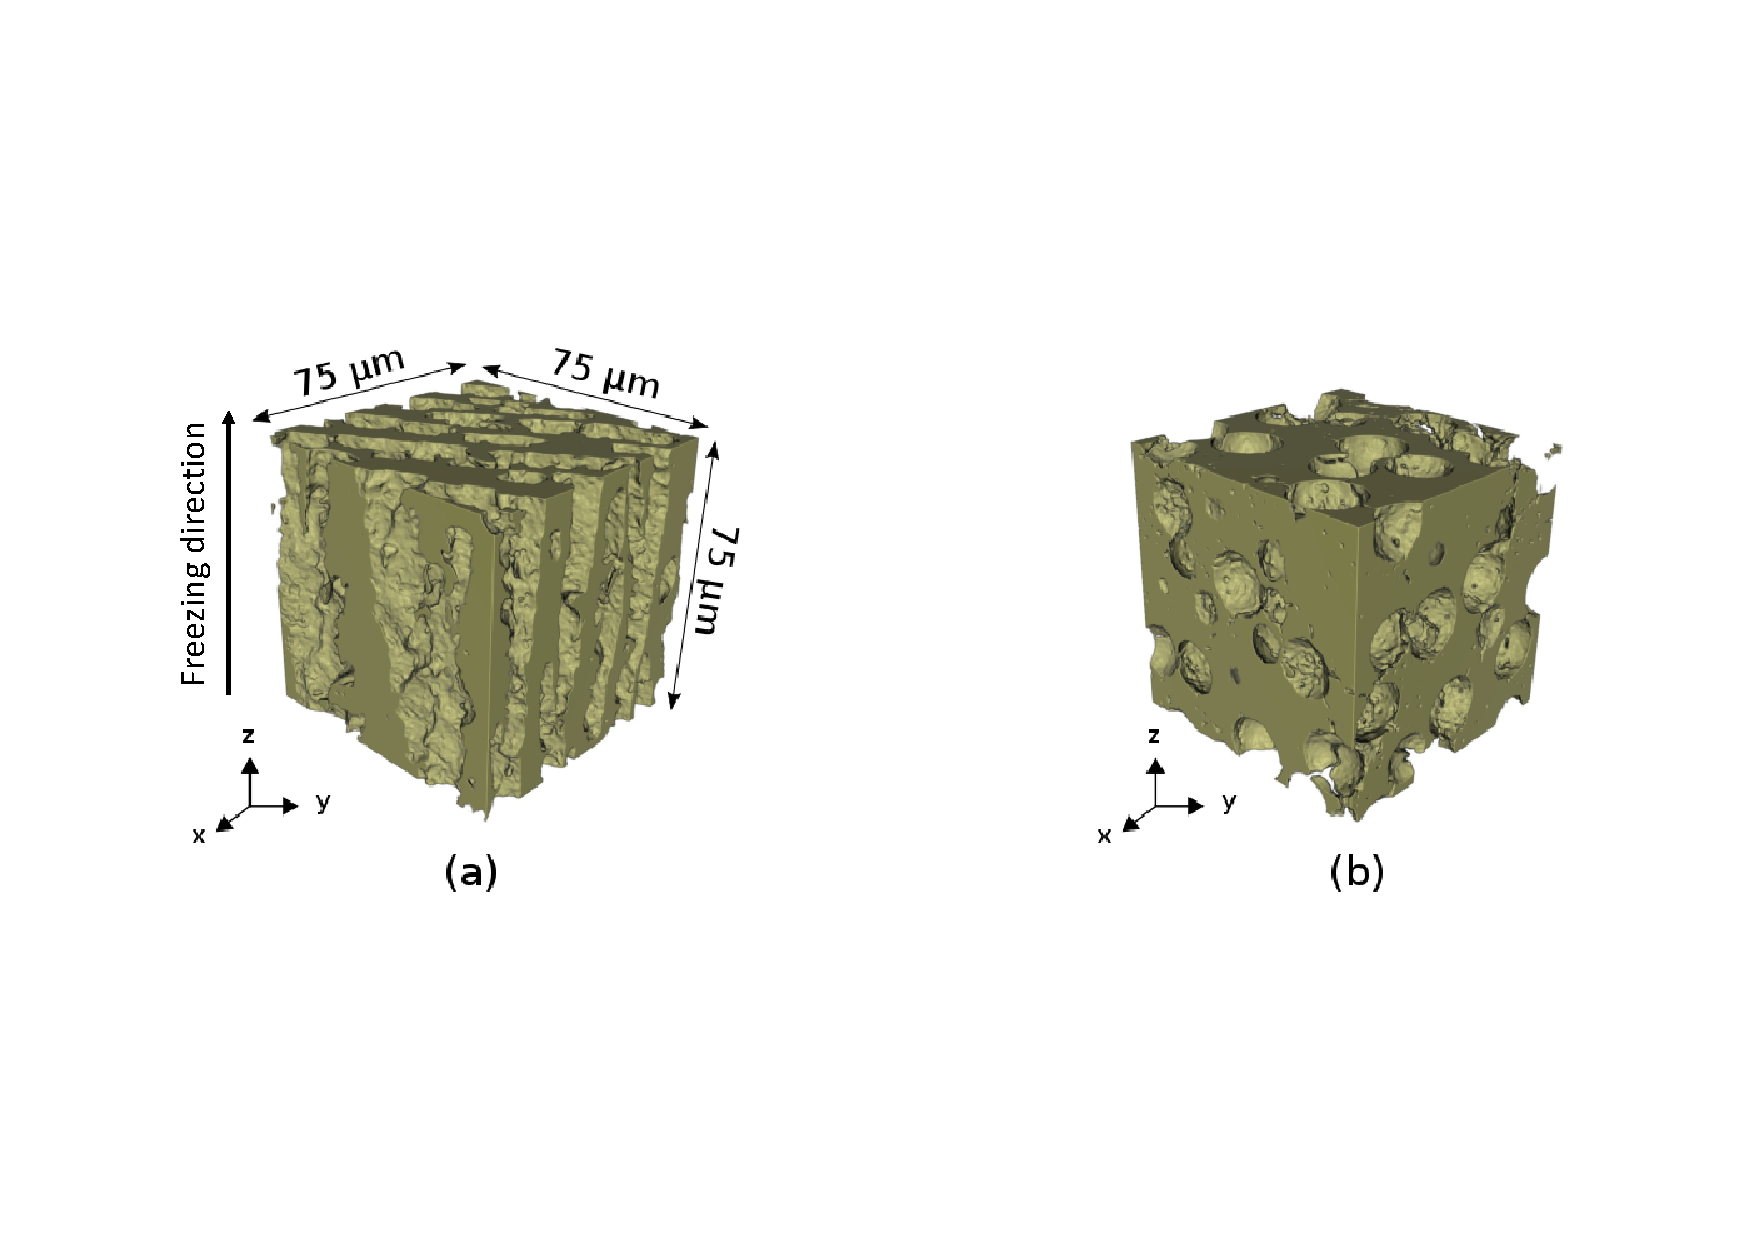
\includegraphics[width=0.95\linewidth{}]{figures/fig1.pdf}
\caption{X-ray nanotomography images  of (a) freeze-cast sample (b) isotropic sample.}
\label{fig1}
\end{figure}

X-ray nanotomography was performed at the nano-imaging end station (ID19) of the European Synchrotron Research Facility (ESRF) to obtain 3D microstructual representations of the anisotropic and isotropic samples \cite{Villanova14} (Fig.~\ref{fig1}). Anisotropic samples (Fig.~\ref{fig1}a) exhibit large pores (macroporosity) aligned with the freezing direction ($z$) with an approximately \SI{10}{\micro\meter} size in the radial direction. The same size is obtained for the isotropic samples (Fig.~\ref{fig1}b), which exhibit a  spherical morphology and narrow size dispersion. The \SI{75}{\nano\meter} resolution attained by X-ray nanotomography is not sufficient to discern the microstructure in the walls. However, SEM micrographs (insert of Fig.~\ref{fig2}a) indicate that the sintering stage produced a partially sintered microstructure with porosity on the order of 25 \% \cite{Lichtner15a}. Coarsening leads to YSZ and LSM particles with approximately \SI{500}{\nano\meter} and \SI{800}{\nano\meter} sizes, respectively. Four anisotropic and two isotropic samples  were imaged. Their total porosity (denoted hereafter $\epsilon$), evaluated by image analysis and confirmed by Archimedes measurements, ranged between 45\% and 68\%, depending on the initial solid loading.  

Numerical microstructures were generated using the nanotomography images. A mixture of spherical particles of 500 nm and 800 nm diameters, representing YSZ and LSM particles, respectively, were first randomly packed into a cubical simulation box with a 60:40 volume ratio. A total of four millions spheres were necessary to obtain a sufficiently large cube to match the scale of the nanotomography images. The numerical packing was subsequently partially sintered to attain 25 \% porosity and create solid bonds between particles~\cite{Jauffres12b}. The packed particle microstructure was then matched with the 3D nanotomography image by removing particles located in the large pores (Fig.~\ref{fig2}b).

The solid bridges that formed during sintering are modeled as elastic bonds, whose size grows in accrordance with Coble's model~\cite{Coble58}. Bonds transmit normal and tangential forces as well as resisting moments. The elastic and fracture properties of the dense material that constitute the bond material are summarized in Table~\ref{table1}. In particular, the bond toughness is approximated as $2\,\gamma_s$, thus modeling a perfectly brittle material. Bonds may fracture in tension or shear when the stress acting on the bond exceeds the bond strength, which is then considered as a crack tip. A fractured bond does not transmit tensile forces but keeps its compressive stiffness. A Coulomb-like law (friction coefficient: 0.5) is installed in shear for broken bonds. A detailed description of the discrete element simulations used here may be found in~\cite{Jauffres12b}. 


\begin{figure}
\centering
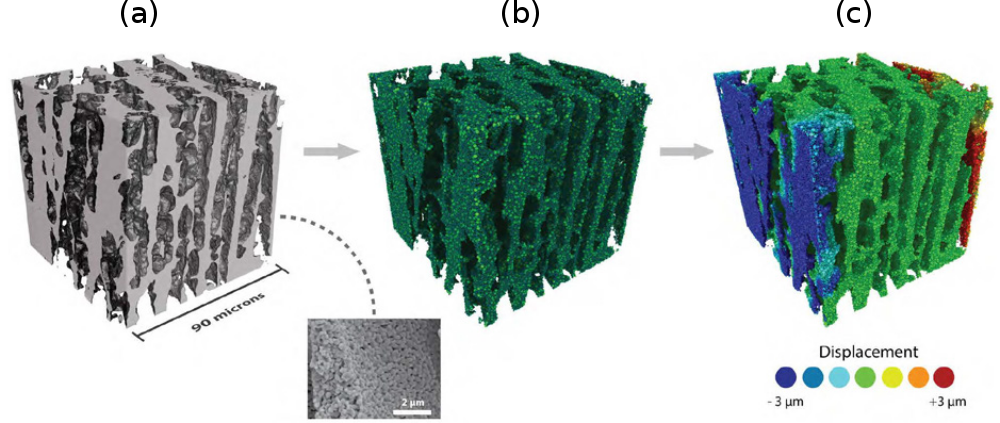
\includegraphics[width=0.95\linewidth{}]{figures/fig2.png}
\caption{Generation of a numerical microstructure from a nanotomagraphy reconstruction using the discrete element method. (a) X-ray nanotomography of a freeze-cast sample. (b) Discrete microstructure matched from the 3D image. (c) Simulation of a crushing test.}
\label{fig2}
\end{figure}


\begin{table}
	\begin{center}
		\begin{tabular}{cccc}
			\hline
				& $E$~\cite{Giraud08,Selcuk97} & $\nu$ & $\gamma_s$~\cite{Kuo05} \\
			\hline
			YSZ & 220 MPa & 0.32 & 0.5~J.m$^{-2}$ \\
			\hline
			LSM & 130 MPa & 0.32 & 0.5~J.m$^{-2}$ \\
			\hline 
			
		\end{tabular}
	\end{center}
	\caption{\label{table1}Material properties of dense particles used for simulations. }
\end{table}

The numerical microstructures were uniaxially crushed with lateral free surfaces (Fig.~\ref{fig2}c). The stress-strain curves were calculated from the total reaction forces on the crushing planes and from the geometry of the crushed samples. Loading-unloading-reloading cycles were imposed to determine the stiffness of the numerical samples during the unloading stages. On such porous microstructures, it is questionable that an elastic reversible domain exists. Thus, we prefer the term stiffness to elastic modulus. The macroscopic strength is also arbitrarily defined as the maximum stress attained during the crushing test (typically attained at $\approx$ 1\% axial strain).

\begin{figure}
\centering
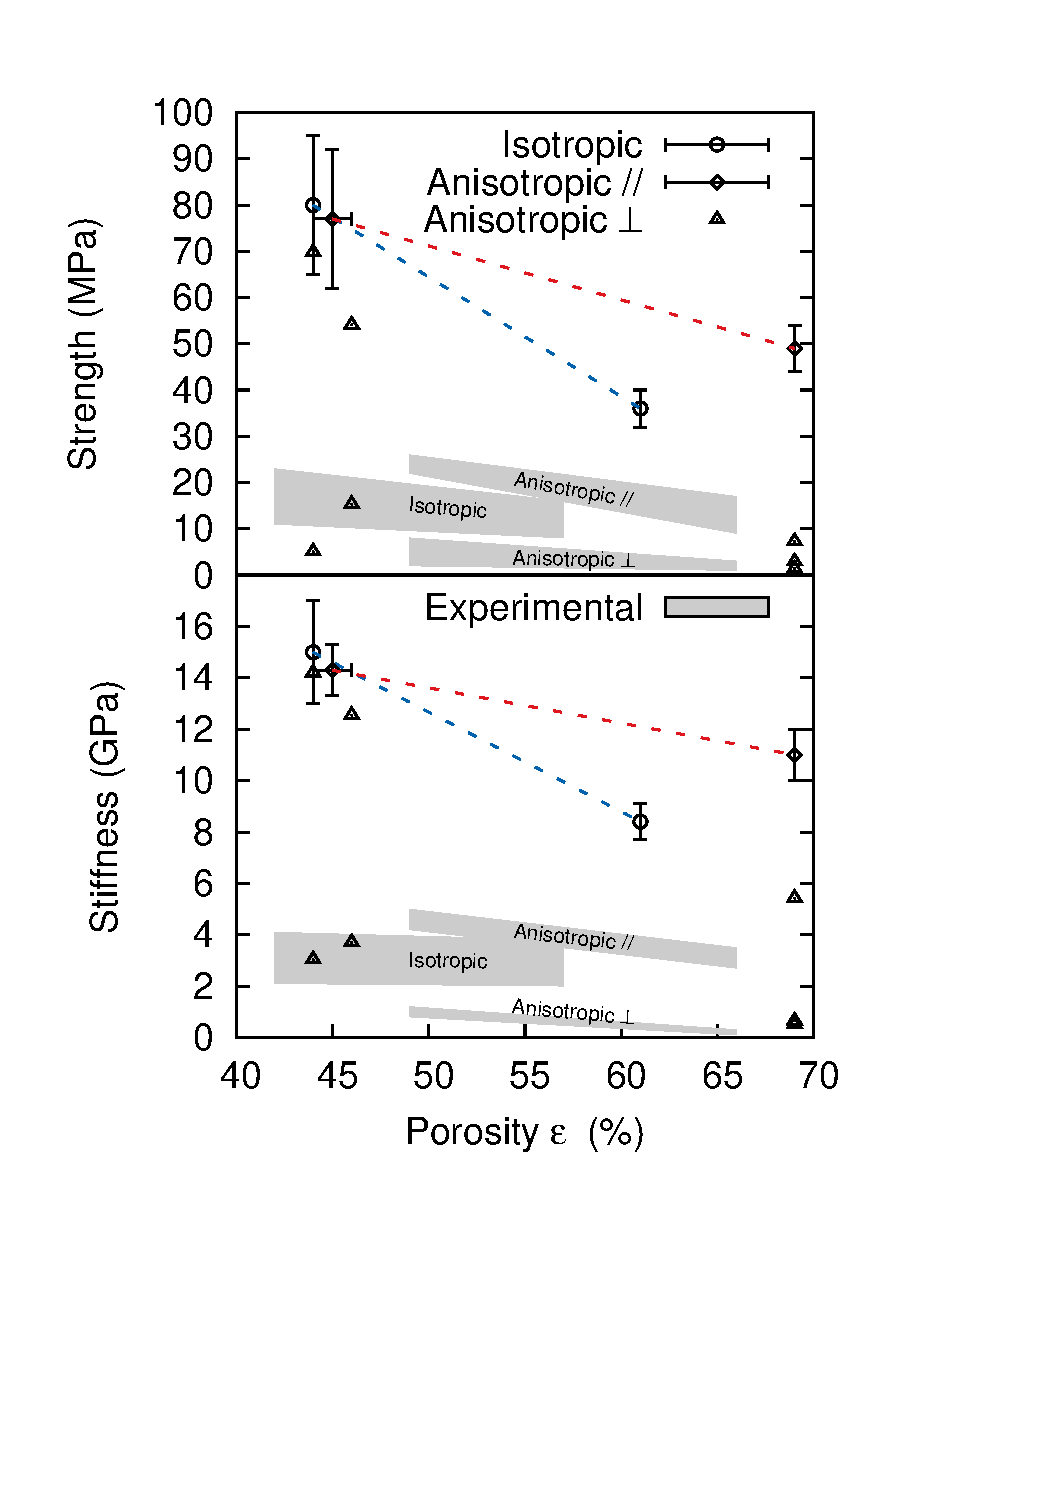
\includegraphics[width=0.6\linewidth{}]{figures/fig3.pdf}
\caption{Strength and stiffness from numerical tests on tomographic images compared with experimental data (shown in grey boxes).}
\label{fig3}
\end{figure}

Freeze-cast samples exhibit anisotropic microstructures (Fig.~\ref{fig1}), which should translate into an anisotropic response. Fig.~\ref{fig3} indicates that for samples with the largest porosity content ($\epsilon \approx$ 68\%), both strength and stiffness are clearly larger for anisotropic samples loaded parallel to the freezing direction. For the lowest porosity content ($\epsilon\approx$ 45\%), strength and stiffness are quite dispersed for anisotropic samples loaded normal to the freezing direction. This may be understood by observing the image of the loaded samples (Figs.~\ref{fig1} and ~\ref{fig2}). Because the 3D image only samples a small fraction of the whole structure, the particular orientations of the walls perpendicular to the freezing direction play a predominant role on the mechanics of the sample. For the whole structure, we have observed that they are randomly oriented with colonies of walls spanning typically over few hundreds of microns. In other words, only the $z$ direction is distinctly anisotropic when considering the whole sample. At low porosity, isotropic samples have similar strength and stiffness than anisotropic ones loaded along the freezing direction, but fall below for large porosity content. 


Fracture mechanisms can be investigated at the particle length scale with discrete simulations. Fig.~\ref{fig4} shows the location of fractured bonds together with large pores just after the stress maximum. The isotropic sample (Fig.~\ref{fig4}a) exhibits a rather heterogeneous distribution of broken bonds, with heavily damaged zones, surrounded by nearly intact ones. However, we observed that the initial damage spreads as cracks (indicated by dotted ellipses) that were more evenly distributed. Anisotropic samples tested parallel to the freezing direction (Fig.~\ref{fig4}b) show damage homogeneously located in the walls. In these samples, damage has expanded in the whole width of the ceramic wall. Conversely, Fig.~\ref{fig4}c indicates that a very small amount of damage is sufficient to crush the sample when the ceramic walls are oriented normal to the loading direction. Note that this sample ($\epsilon\approx$ 0.69) is associated with an extremely low strength (1.4 MPa), as it should.


Fig.~\ref{fig3} also includes experimental data on macroscopic rectangular samples (12mm $\times$ 12mm $\times$ 16mm) which were crushed under similar conditions \cite{Lichtner15b}. It is clear that simulation results lead to an overestimation both of strength and stiffness. We have not attempted to fit any material parameter in the model (Young's moduli and surface energies of LSM and YSZ are directly taken from literature, see table~\ref{table1}). Previous comparisons with experimental data for partially sintered ceramics (no templated macroporosity) lead to very good agreement for elasticity \cite{Jauffres12MSMSE}. As for strength, an overestimation by a factor of 2 was attributed to the absence in the ideal numerical microstructure of some kind of initial flaw for fracture \cite{Jauffres13}. In the present case, the simulated microstructure is very close to the real one but the simulated volume is an issue. Classical Weibull statistics tells us that strength depends on the length of the major flaw and that the probability of failure increases with the size of the specimen. According to Weibull statistics, the probability of failure in a sample of volume $V_1$ is equal to that in a sample of volume $V_2$ if stresses $\sigma_1$ and $\sigma_2$ are related by:
\begin{equation}
V_1 \sigma_1^m=V_2 \sigma_2^m \label{eqn1}
\end{equation}
where $m$ is the Weibull modulus that measures the scatter of strength data. Eq.~(\ref{eqn1}) assumes that a single flaw type population initiates failure whatever the specimen size \cite{Danzer08}. A full Weibull statistics is out of reach with our limited data. Still, it is interesting to note that Eq.~(\ref{eqn1}) leads to $m\approx 9$ for the isotropic microstructure, which is in very good accordance with the experimental values collected by Keles et al. \cite{Keles13} on numerous porous ceramics within the porosity range studied here.

Although Eq.~(\ref{eqn1}) explains rather well the volume dependence for the strength data, it can only suggest that some fracture mechanisms are also at play very early on during the deformation of the samples. This would also explain the stiffness dependence on volume. This is well corroborated by our observation that in simulations, although bonds break predominantly just before the stress maximum is attained, some bonds do break quite early. This indicates that for such highly porous materials, it is not possible to define an elastic core. 



\begin{figure}
\centering
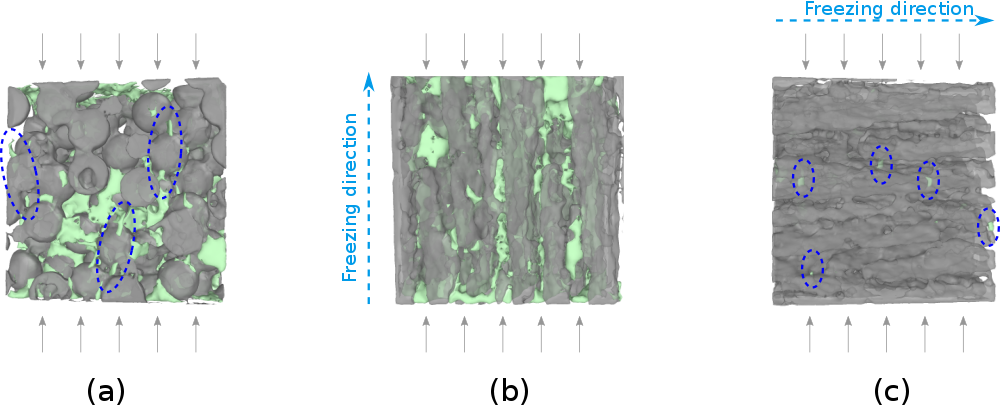
\includegraphics[width=0.95\linewidth{}]{figures/fig4.png}
\caption{Fractured bonds after crushing for an isotropic (a) sample ($\epsilon=0.61$) and for an anisotropic sample loaded parallel (b) and normal (c) to the freezing direction. Macropores are in light gray and clusters of fractured bonds are green.}
\label{fig4}
\end{figure}

The authors thank the National Science Foundation (NSF, grant no. 1008600) and the French National Research Agency (ANR, grant no. 2010 BLAM 0931 01).

%% The Appendices part is started with the command \appendix;
%% appendix sections are then done as normal sections
%\appendix
%
%\section{Section in Appendix}
%\label{appendix-sec1}

%% References
%%
%% Following citation commands can be used in the body text:
%% Usage of \cite is as follows:
%%   \cite{key}         ==>>  [#]
%%   \cite[chap. 2]{key} ==>> [#, chap. 2]
%%

%% References with bibTeX database:

\bibliographystyle{elsarticle-num}
% \bibliographystyle{elsarticle-harv}
% \bibliographystyle{elsarticle-num-names}
% \bibliographystyle{model1a-num-names}
% \bibliographystyle{model1b-num-names}
% \bibliographystyle{model1c-num-names}
% \bibliographystyle{model1-num-names}
% \bibliographystyle{model2-names}
% \bibliographystyle{model3a-num-names}
% \bibliographystyle{model3-num-names}
% \bibliographystyle{model4-names}
% \bibliographystyle{model5-names}
% \bibliographystyle{model6-num-names}

%\bibliography{library}
\begin{thebibliography}{10}
\expandafter\ifx\csname url\endcsname\relax
  \def\url#1{\texttt{#1}}\fi
\expandafter\ifx\csname urlprefix\endcsname\relax\def\urlprefix{URL }\fi
\expandafter\ifx\csname href\endcsname\relax
  \def\href#1#2{#2} \def\path#1{#1}\fi

\bibitem{Laurencin12}
J.~Laurencin, R.~Quey, G.~Delette, H.~Suhonen, P.~Cloetens, P.~Bleuet, J. Power Sources
  198 (2012) 182.
\bibitem{Zhang12b}
L.~Zhang, J.~M.~F. Ferreira, S.~Olhero, L.~Courtois, T.~Zhang, E.~Maire,
  J.~C.~Rauhe,  Acta Mater. 60 (2012) 4235.
\bibitem{Lichtner13}
A.~Z. Lichtner, D.~Jauffr\`{e}s, C.~L. Martin, R.~K. Bordia, J. Am. Ceram. Soc. 96
  (2013) 2745.
\bibitem{Lichtner15a}
A.~Z. Lichtner, D.~Jauffr\`{e}s, D.~Roussel, F.~Charlot, C.~L. Martin, R.~K.
  Bordia, Journal of the European Ceramic Society 35
  (2015) 585.
  \bibitem{Lichtner15b}
A.~Lichtner, D.~Roussel, C.~L. Martin, R.~K. Bordia,  submitted.
\bibitem{Villanova14}
J.~Villanova, P.~Cloetens, H.~Suhonen, J.~Laurencin, F.~Usseglio-Viretta,
  E.~Lay, G.~Delette, P.~Bleuet, D.~Jauffr\`{e}s, D.~Roussel, A.~Z. Lichtner,
  C.~L. Martin, Journal of Materials Science 49 (2014) 5626.
\bibitem{Jauffres12b}
D.~Jauffr\`{e}s, C.~L. Martin, A.~Lichtner, R.~K. Bordia,
  Acta Mater. 60 (2012) 4685.
\bibitem{Coble58}
R.~L. Coble,J. Am. Ceram. Soc. 41 (1958) 55.
\bibitem{Giraud08}
S.~Giraud, J.~Canel, J. Eur. Ceram. Soc. 28 (2008) 77.
\bibitem{Selcuk97}
A.~Sel\c{c}uk, A.~Atkinson,  J. Eur. Ceram. Soc. 17 (1997) 1523.
\bibitem{Kuo05}
C.-W. Kuo, Y.-H. Lee, K.-Z. Fung, M.-C. Wang, J. Non-Cryst. Solids 351 (2005) 304.
\bibitem{Liu11}
X.~Liu, C.~L. Martin, D.~Bouvard, S.~D. Iorio, J.~Laurencin, G.~Delette, J. Am. Ceram. Soc. 94 (2011) 3500.
\bibitem{Danzer08}
R.~Danzer, T.~Lube, P.~Supancic, R.~Damani, Adv. Eng.  Mater. 10 (2008) 275.
\bibitem{Keles13}
O.~Keles, R.~E. Garcia, K.~J. Bowman, Acta Mater. 61 (2013) 2853.
\bibitem{Elices02}
M.~Elices, G.V.~Guinea, J.~Gómez, J.~Planas, Engineering Fracture Mechanics 69 (2002) 137.
\bibitem{Jauffres12MSMSE}
D.~Jauffrès, C.~L. Martin, A.~Lichtner, R.~K. Bordia, Modelling and Simulation in Materials Science and Engineering, 20 (2012)
\bibitem{Jauffres13}
D.~Jauffrès, X.~Liu, C.~L. Martin, Engineering Fracture Mechanics, 103 (2013) 132.
\end{thebibliography}


\end{document}

%%
%% End of file `elsarticle-template-num.tex'.
